\setcounter{page}{1}


\section{Introducción}
    Ejemplo de cita~(\cite{buffett84}).
\section{Objetivos}
    \begin{itemize}
        \item Implementar VLAN de acceso.
        \item Identicar IP's con clase.
    \end{itemize}

\section{Desarrollo del Trabajo}

    \begin{table}[H]
        \begin{center}
            \begin{tabular}{ c | c | c | c }
                \textbf{VLAN} & \textbf{Nombre} & \textbf{Puertos} & \textbf{Red}\\ \hline
                2 & ELECTRONICA & 2,4,6,8 & 1.0.0.0/8\\
                4 & SISTEMAS & 10,12,14,16 & 10.0.0.0/8\\
                6 & CIVIL & 1,3,5,7 & 172.16.0.0/16\\
                8 & ELECTRICA & 9,11,13,15 & 192.168.6.0/24\\
            \end{tabular}
            \caption{VLAN's}
            \label{tab:VLANs}
            \end{center}
    \end{table}

    \subsection{Configuración de las VLAN's en Cisco Packet Tracer PC1}
        Para comenzar a configurar, en el simulador agregamos un Switch, 4 servidores y 12 PC's. Posteriormente, procedemos a conectar los dispositivos de acuerdo al puerto asignado en la tabla~\ref{tab:VLANs}, según la VLAN a la que se desea asignar. En la figura~\ref{fig:cisco} se muestra la configuración en el simulador Cisco Packet Tracer.

        \begin{figure}[H]
            \centering
            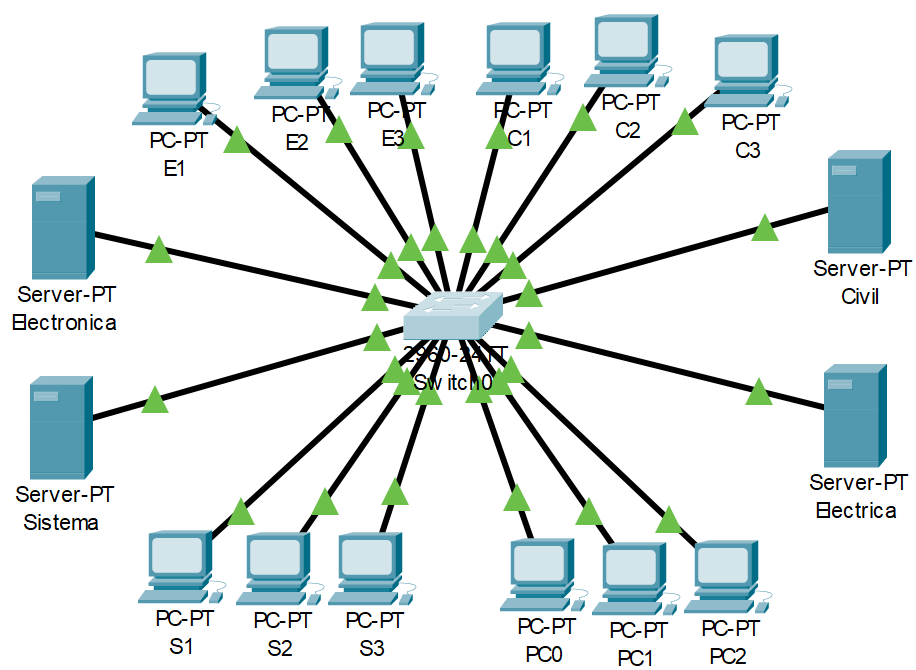
\includegraphics[width=0.6\textwidth]{img/cisco.png}
            \caption{Configuración en el simulador Cisco Packet Tracer}
            \label{fig:cisco}
        \end{figure}

        Para configurar la VLAN 2 en el switch y asignar los puertos correspondientes al departamento de Electrónica, es necesario acceder a la terminal del switch y ejecutar los siguientes comandos:

        \begin{lstlisting}[language=bash, caption={Creación y configuración de la VLAN 2},label={lst:cisco_vlan2}]
            Switch(config)# vlan 2
            Switch(config-vlan)# name ELECTRONICA
            Switch(config)# interface range fa0/2, fa0/4, fa0/6, fa0/8
            Switch(config-if-range)# switchport mode access
            Switch(config-if-range)# switchport access vlan 2
        \end{lstlisting}

        Para configurar la VLAN 4 en el switch y asignar los puertos correspondientes al departamento de Sistemas, es necesario acceder a la terminal del switch y ejecutar los siguientes comandos:

        \begin{lstlisting}[language=bash, caption={Creación y configuración de la VLAN 4},label={lst:cisco_vlan4}]
            Switch(config)# vlan 4
            Switch(config-vlan)# name SISTEMAS
            Switch(config)# interface range fa0/10, fa0/12, fa0/14, fa0/16
            Switch(config-if-range)# switchport mode access
            Switch(config-if-range)# switchport access vlan 4
        \end{lstlisting}

        Para configurar la VLAN 6 en el switch y asignar los puertos correspondientes al departamento de Civil, es necesario acceder a la terminal del switch y ejecutar los siguientes comandos:

        \begin{lstlisting}[language=bash, caption={Creación y configuración de la VLAN 6},label={lst:cisco_vlan6}]
            Switch(config)# vlan 6
            Switch(config-vlan)# name CIVIL
            Switch(config)# interface range fa0/1, fa0/3, fa0/5, fa0/7
            Switch(config-if-range)# switchport mode access
            Switch(config-if-range)# switchport access vlan 6
        \end{lstlisting}

        Finalmente, para configurar la VLAN 8 en el switch y asignar los puertos correspondientes al departamento de Eléctrica, es necesario acceder a la terminal del switch y ejecutar los siguientes comandos:

        \begin{lstlisting}[language=bash, caption={Creación y configuración de la VLAN 8},label={lst:cisco_vlan8}]
            Switch(config)# vlan 8
            Switch(config-vlan)# name ELECTRICA
            Switch(config)# interface range fa0/9, fa0/11, fa0/13, fa0/15
            Switch(config-if-range)# switchport mode access
            Switch(config-if-range)# switchport access vlan 8
        \end{lstlisting}

        En la figura~\ref{fig:cisco_vlan_PC1} se muestra la configuración de todos los VLAN's en el Switch del simulador Cisco Packet Tracer.

        \begin{figure}[H]
            \centering
            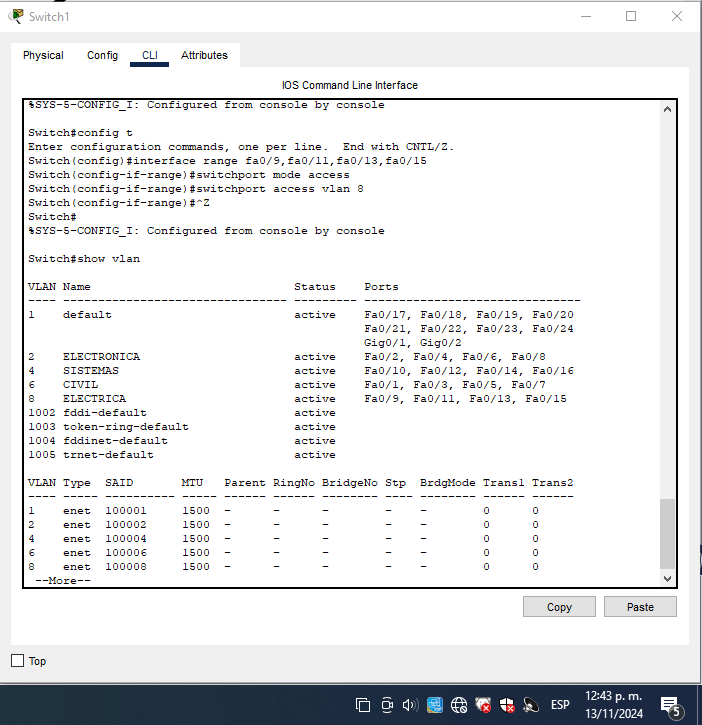
\includegraphics[width=0.6\textwidth]{img/cisco_vlan_PC1.png}
            \caption{Configuración de todos los VLAN's en el Switch del simulador Cisco Packet Tracer}
            \label{fig:cisco_vlan_PC1}
        \end{figure}

        Para probar la configuración de las VLAN's, se ingresó a la página web de cada servidor desde las PC's asignadas a cada departamento. La dirección IP de cada servidor se muestra en la tabla~\ref{tab:IPs}.

        \begin{table}[H]
            \begin{center}
                \begin{tabular}{ c | c | c | c }
                    \textbf{VLAN perteneciente} & \textbf{Servidor} & \textbf{Dirección IP} & \textbf{Máscara de subred}\\ \hline
                    2 & Electrónica & 1.0.0.100 & 255.0.0.0\\
                    4 & Sistemas & 10.0.0.100 & 255.0.0.0\\
                    6 & Civil & 172.16.0.100 & 255.255.0.0\\
                    8 & Eléctrica & 192.168.6.100 & 255.255.255.0\\
                \end{tabular}
                \caption{Direcciones IP de los servidores}
                \label{tab:IPs}
                \end{center}
        \end{table}

        Desde la PC E1, el cual pertenece al departamento de Electrónica, se ingresó a la página web del servidor, cuya dirección IP es \texttt{1.0.0.100} como se muestra en la figura~\ref{fig:servidor_electronica_PC1}.

        \begin{figure}[H]
            \centering
            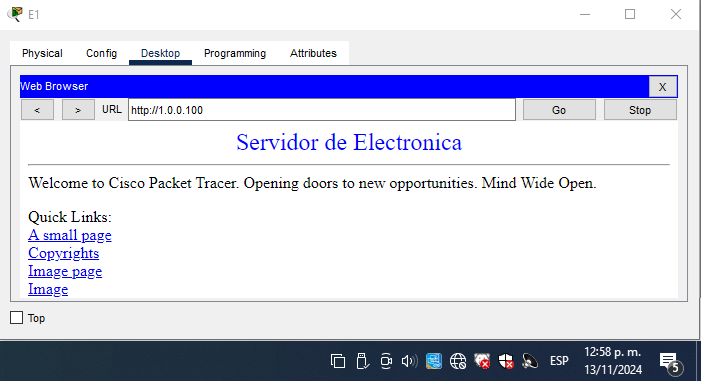
\includegraphics[width=0.7\textwidth]{img/servidor_electronica_PC1.png}
            \caption{Página web del servidor de Electrónica}
            \label{fig:servidor_electronica_PC1}
        \end{figure}

        Desde la PC S1, el cual pertenece al departamento de Sistemas, se ingresó a la página web del servidor, cuya dirección IP es \texttt{10.0.0.100} como se muestra en la figura~\ref{fig:servidor_sistemas_PC1}.

        \begin{figure}[H]
            \centering
            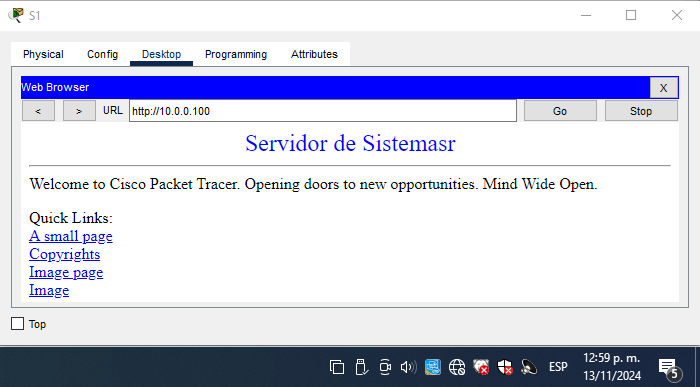
\includegraphics[width=0.7\textwidth]{img/servidor_sistemaPC1.png}
            \caption{Página web del servidor de Sistemas}
            \label{fig:servidor_sistemas_PC1}
        \end{figure}

        Desde la PC C1, el cual pertenece al departamento de Civil, se ingresó a la página web del servidor, cuya dirección IP es \texttt{172.16.0.100} como se muestra en la figura~\ref{fig:servidor_civil_PC1}.

        \begin{figure}[H]
            \centering
            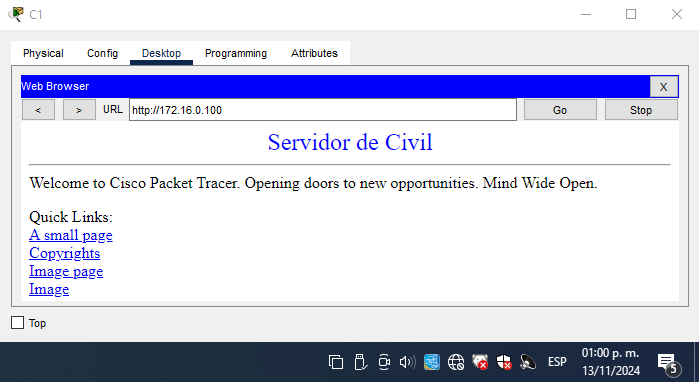
\includegraphics[width=0.7\textwidth]{img/servidor_civil_PC1.png}
            \caption{Página web del servidor de Civil}
            \label{fig:servidor_civil_PC1}
        \end{figure}

        Desde la PC1, el cual pertenece al departamento de Eléctrica, se ingresó a la página web del servidor, cuya dirección IP es \texttt{192.168.6.100} como se muestra en la figura~\ref{fig:servidor_electrica_PC1}.

        \begin{figure}[H]
            \centering
            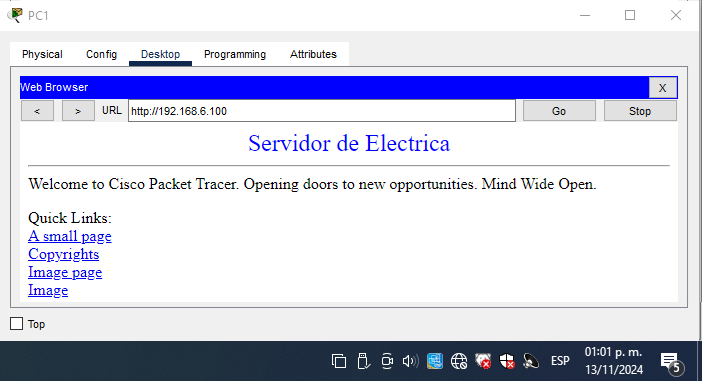
\includegraphics[width=0.7\textwidth]{img/servidor_electrica_PC1.png}
            \caption{Página web del servidor de Eléctrica}
            \label{fig:servidor_electrica_PC1}
        \end{figure}

        Cada PC se conectó a la página web del servidor correspondiente a su departamento, lo que indica que la configuración de las VLAN's fue exitosa.

    \subsection{Configuración de las VLAN's en el Switch}
        


        \begin{figure}[H]
            \centering
            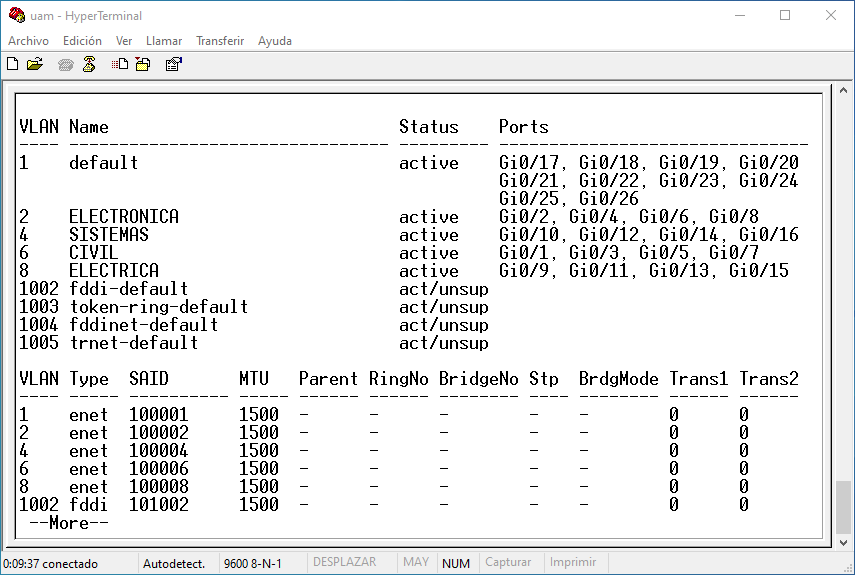
\includegraphics[width=0.7\textwidth]{img/vlansSwitch.png}
            \caption{VLAN's creadas en el Switch}
            \label{fig:vlansSwitch}
        \end{figure}

        \begin{figure}[H]
            \centering
            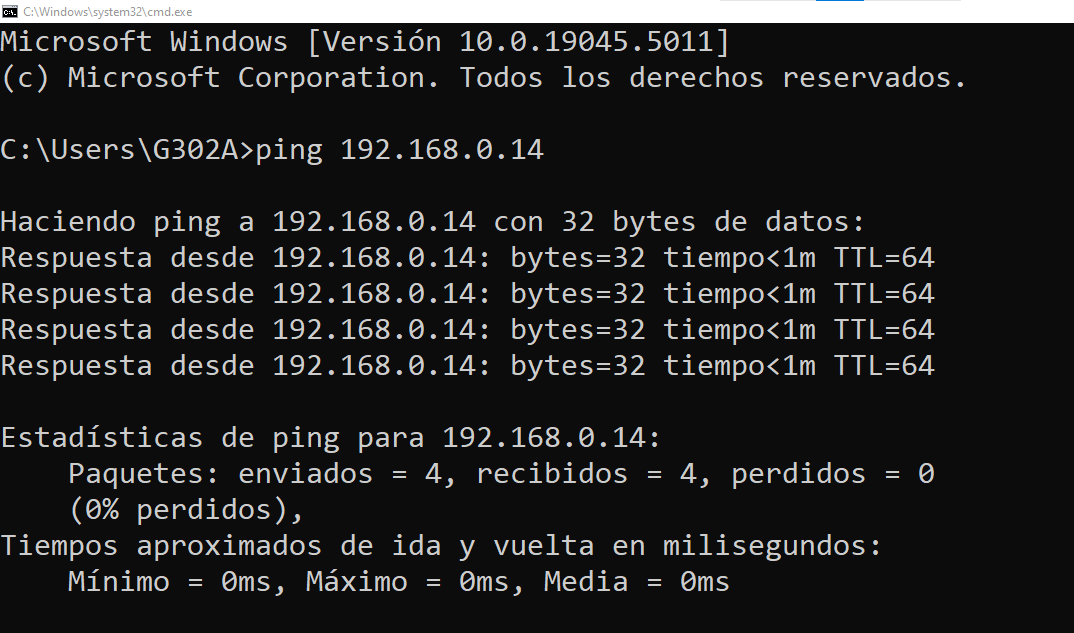
\includegraphics[width=0.7\textwidth]{img/ping_default.png}
            \caption{VLAN default en el Switch}
            \label{fig:ping_default}
        \end{figure}


        \begin{figure}[H]
            \centering
            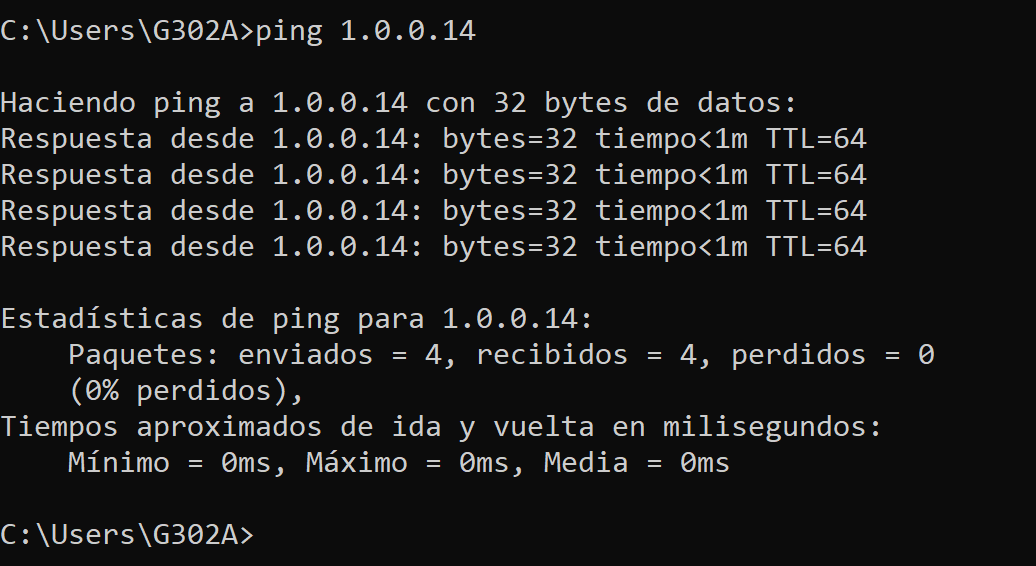
\includegraphics[width=0.7\textwidth]{img/ping_vlan2.png}
            \caption{VLAN 2 en el Switch}
            \label{fig:ping_vl an2}
        \end{figure}


        \begin{figure}[H]
            \centering
            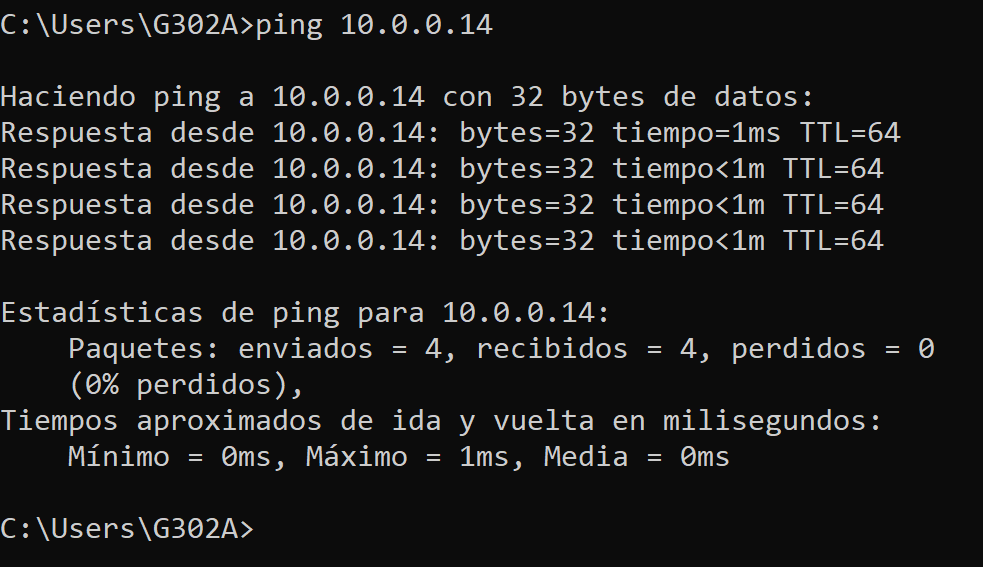
\includegraphics[width=0.7\textwidth]{img/ping_vlan4.png}
            \caption{VLAN 4 en el Switch}
            \label{fig:ping_vlan4}
        \end{figure}


        \begin{figure}[H]
            \centering
            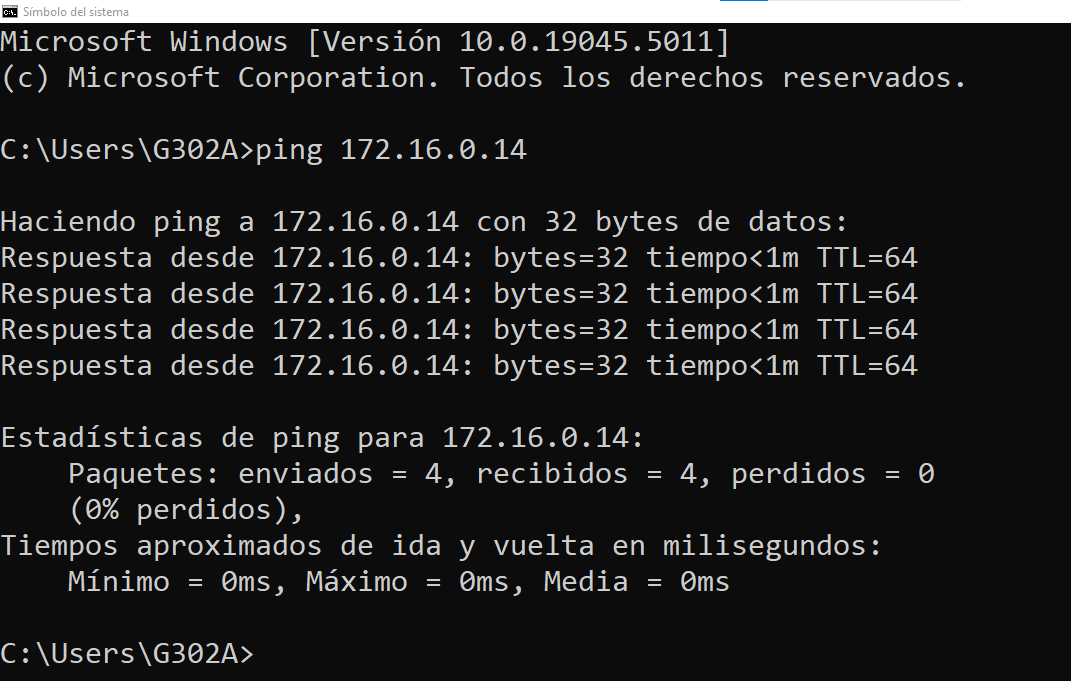
\includegraphics[width=0.7\textwidth]{img/ping_vlan6.png}
            \caption{VLAN 6 en el Switch}
            \label{fig:ping_vlan6}
        \end{figure}

        \begin{figure}[H]
            \centering
            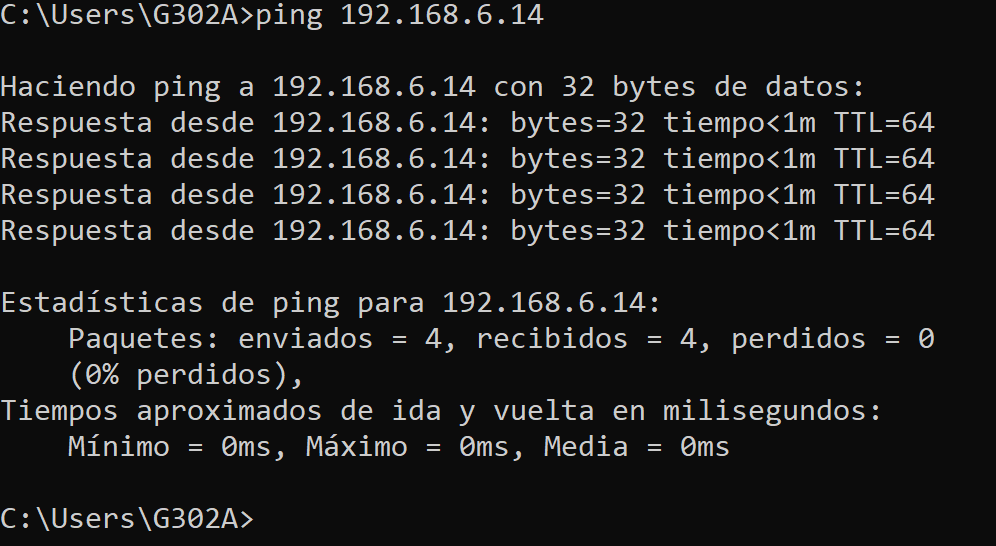
\includegraphics[width=0.7\textwidth]{img/ping_vlan8.png}
            \caption{VLAN 8 en el Switch}
            \label{fig:ping_vlan8}
        \end{figure}


\section{Conclusiones}

% --- Para agregar un apéndice
%\newpage
%\appendix
%\appendixpage
%\addappheadtotoc
%\section{Nombre del apéndice}